
\documentclass[12pt, onecolumn]{IEEEtran}
%\documentclass{article}
\usepackage[utf8]{inputenc}
\usepackage[T1]{fontenc}
\usepackage{lmodern}
\usepackage{graphicx}
\usepackage{color}
\usepackage{hyperref}
\usepackage{amsmath}
\usepackage{amsfonts}
\usepackage{epstopdf}
\usepackage[table]{xcolor}
\usepackage{matlab}
\usepackage{amssymb}
\usepackage{latexsym}
\usepackage{epsfig}
%\usepackage{comp}
\usepackage{algorithm}
\usepackage{algorithmic}

\begin{document}
	\author{Athar Ali (22915030)}
	\title{\bf{ \large EEN - 521 Digital Signal and Image Processing\\ Lab Report 1}}
	\maketitle 
	\markboth{\small \it{D\lowercase{epartment of} E\lowercase{lectrical} E\lowercase {ngineering}}  \hfill A\lowercase{utumn} S\lowercase{emester 
			2022} } {}
	
	%\matlabheading{EEN - 521 Digital Signal and Image Processing}
	
	
	\vspace{1em}
	\begin{par}
		\begin{flushleft}
			\textbf{1) Generate the following sequences in MATLAB:}
		\end{flushleft}
	\end{par}
	
	\begin{par}
		\begin{flushleft}
			\textbf{a) An impulse at t = 0} 
		\end{flushleft}
	\end{par}
	
	\begin{matlabcode}
		clc;
		n=-5:5;
		n0=input('Enter the Location of impulse = ')
	\end{matlabcode}
	\begin{matlaboutput}
		n0 = 0
	\end{matlaboutput}
	\begin{matlabcode}
		del= [n-n0==0];
		display(del,'Sequence');
	\end{matlabcode}
	\begin{matlaboutput}
		Sequence = 1x11 logical array    
		0   0   0   0   0   1   0   0   0   0   0
		
	\end{matlaboutput}
	\begin{matlabcode}
		display(n, 'Idices')
	\end{matlabcode}
	\begin{matlaboutput}
		Idices = 1x11    
		-5    -4    -3    -2    -1     0     1     2     3     4     5
		
	\end{matlaboutput}
	\begin{matlabcode}
		figure;
		stem(n,del,'linewidth',2,'color','b'); grid
		title("Impulse function at t=0")
		xlabel("Indices")
		ylabel("Magnitude")
		xlim([-5 5])
		ylim([-1 2])
	\end{matlabcode}
	\begin{center}
		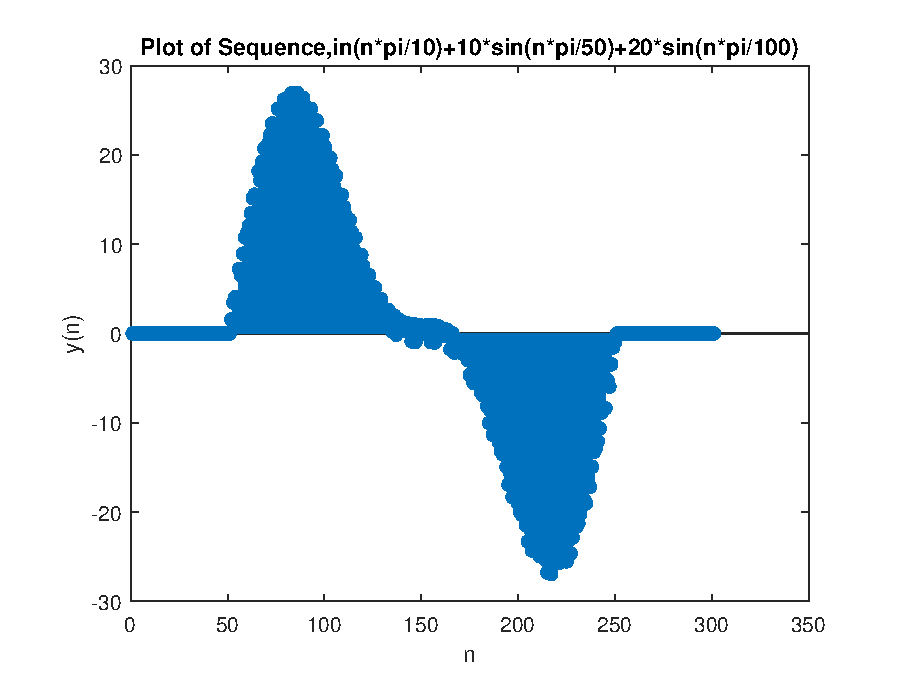
\includegraphics[width=\maxwidth{56.196688409433015em}]{figure_0.eps}
	\end{center}
	
	\begin{par}
		\begin{flushleft}
			\textbf{b) Unit step sequence of length N}
		\end{flushleft}
	\end{par}
	
	\begin{matlabcode}
		N=input('Enter the Length of Unit Step Sequence = ')
	\end{matlabcode}
	\begin{matlaboutput}
		N = 10
	\end{matlaboutput}
	\begin{matlabcode}
		n1=-N/2:N/2-1
	\end{matlabcode}
	\begin{matlaboutput}
		n1 = 1x10    
		-5    -4    -3    -2    -1     0     1     2     3     4
		
	\end{matlaboutput}
	\begin{matlabcode}
		u= [(n1-0) >= 0];
		display(u,'Sequence');
	\end{matlabcode}
	\begin{matlaboutput}
		Sequence = 1x10 logical array    
		0   0   0   0   0   1   1   1   1   1
		
	\end{matlaboutput}
	\begin{matlabcode}
		display(n1, 'Idices')
	\end{matlabcode}
	\begin{matlaboutput}
		Idices = 1x10    
		-5    -4    -3    -2    -1     0     1     2     3     4
		
	\end{matlaboutput}
	\begin{matlabcode}
		figure;
		stem(n1,u,'linewidth',2,'color','k'); grid
		title(" Unit step sequence of length N")
		xlabel("Indices")
		ylabel("Magnitude")
		ylim([-1 2])
	\end{matlabcode}
	\begin{center}
		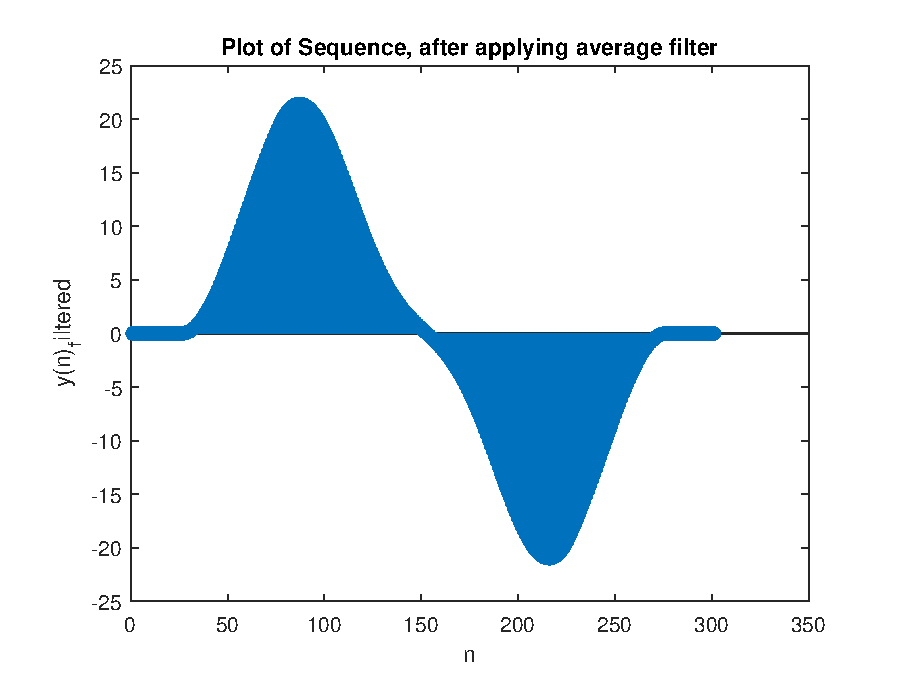
\includegraphics[width=\maxwidth{56.196688409433015em}]{figure_1.eps}
	\end{center}
	\begin{matlabcode}
		
	\end{matlabcode}
	
	\begin{par}
		\begin{flushleft}
			\textbf{c) Ramp signal of length N and slope S.}
		\end{flushleft}
	\end{par}
	
	\begin{matlabcode}
		s=input('Enter the Slop of Ramp, s = ');
		ramp = s*n1.*u;
		display(ramp,'Sequence');
	\end{matlabcode}
	\begin{matlaboutput}
		Sequence = 1x10    
		0     0     0     0     0     0     2     4     6     8
		
	\end{matlaboutput}
	\begin{matlabcode}
		display(n1, 'Idices')
	\end{matlabcode}
	\begin{matlaboutput}
		Idices = 1x10    
		-5    -4    -3    -2    -1     0     1     2     3     4
		
	\end{matlaboutput}
	\begin{matlabcode}
		figure
		stem(n1,ramp,'linewidth',2,'color','r'); grid
		title("  Ramp signal of length N and slope s")
		xlabel("Indices")
		ylabel("Magnitude")
	\end{matlabcode}
	\begin{center}
		\includegraphics[width=\maxwidth{56.196688409433015em}]{figure_2.eps}
	\end{center}
	
	\begin{par}
		\begin{flushleft}
			\textbf{d)} $\mathbf{x(n)=2\delta (n+2)-\delta(n-4), -5\leq n\leq5}$
		\end{flushleft}
	\end{par}
	
	\begin{matlabcode}
		n = -5:5;
		xn = 2*((n+2)==0)-((n-4)==0); % The delta function
		display(xn,'Sequence');
	\end{matlabcode}
	\begin{matlaboutput}
		Sequence = 1x11    
		0     0     0     2     0     0     0     0     0    -1     0
		
	\end{matlaboutput}
	\begin{matlabcode}
		display(n, 'Idices')
	\end{matlabcode}
	\begin{matlaboutput}
		Idices = 1x11    
		-5    -4    -3    -2    -1     0     1     2     3     4     5
		
	\end{matlaboutput}
	\begin{matlabcode}
		figure;
		stem(n,xn,'linewidth',2,'color','b'); grid
		
		xlabel("Indices")
		ylabel("Magnitude")
		ylim([-2 3])
	\end{matlabcode}
	\begin{center}
		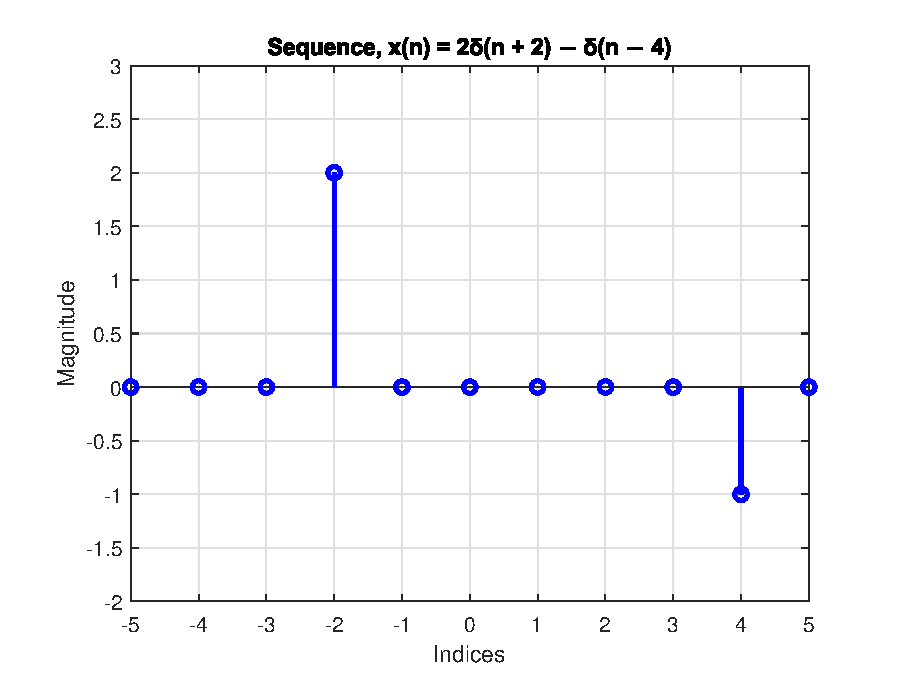
\includegraphics[width=\maxwidth{56.196688409433015em}]{figure_3.eps}
	\end{center}
	
	\begin{par}
		\begin{flushleft}
			\textbf{e)} $\mathbf{x(n) = cos(0.04\pi n) + 0.2w(n), 0 \leq  n \leq 50,}$ \textbf{where w(n) is a Gaussian sequence with zero mean and unit variance.}
		\end{flushleft}
	\end{par}
	
	\begin{matlabcode}
		mu=input('Enter the value of mean = ');
		var=input('Enter the value of Variation = ');
		sigma=sqrt(var)
	\end{matlabcode}
	\begin{matlaboutput}
		sigma = 1
	\end{matlaboutput}
	\begin{matlabcode}
		xn=1:50;
		pdf = @(x) (1/sqrt(2*sigma^2))*exp((-(x-mu).^2)/(2*sigma^2));
		figure
		subplot(311)
		fplot(pdf,  [0 50]); grid
		cos_f = @(x) cos(0.04*pi*x)
	\end{matlabcode}
	\begin{matlaboutput}
		cos_f = 
		@(x)cos(0.04*pi*x)
		
	\end{matlaboutput}
	\begin{matlabcode}
		subplot(312)
		fplot(cos_f, [0 50]); grid
		xn =@(x) cos_f + pdf
	\end{matlabcode}
	\begin{matlaboutput}
		xn = 
		@(x)cos_f+pdf
		
	\end{matlaboutput}
	\begin{matlabcode}
		$xn1 =@(x) cos(0.04*pi*x) + 0.2*(1/sqrt(2*sigma^2))*exp((-(x-mu).^2)/(2*sigma^2));$
		subplot(313)
		fplot(xn1, [0 50]); grid
	\end{matlabcode}
	\begin{center}
		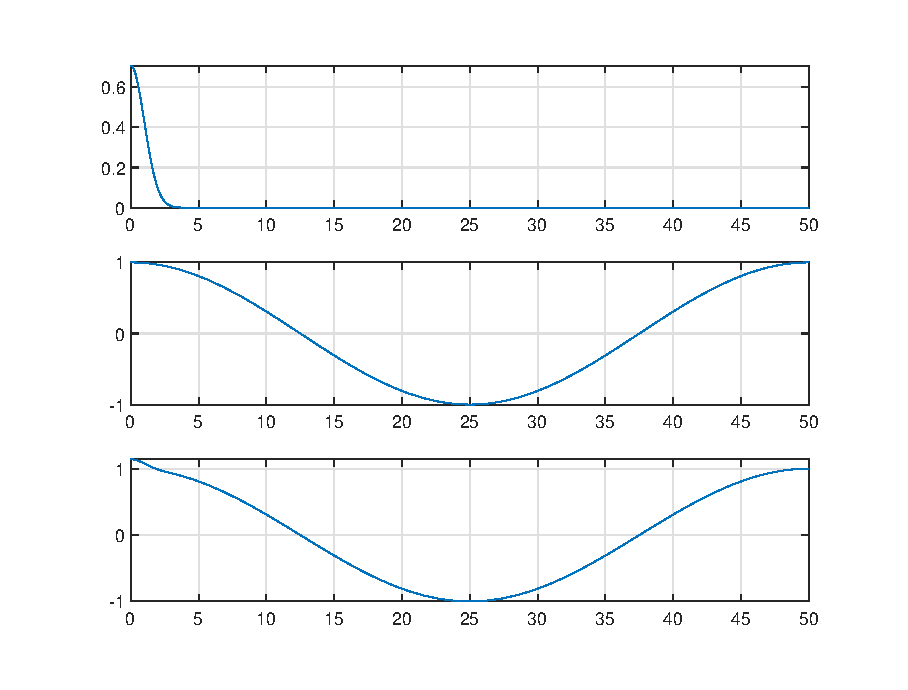
\includegraphics[width=\maxwidth{56.196688409433015em}]{figure_4.eps}
	\end{center}
	
	\begin{par}
		\begin{flushleft}
			\textbf{2nd Method}
		\end{flushleft}
	\end{par}
	
	\begin{matlabcode}
		n = 0:50; 
		xn = cos(0.04*pi*n)+0.2*randn(size(n));
		figure
		stem(n,xn); grid
		title('Sequence in Problem 2.1c')
		xlabel('n'); 
		ylabel('x(n)');
	\end{matlabcode}
	\begin{center}
		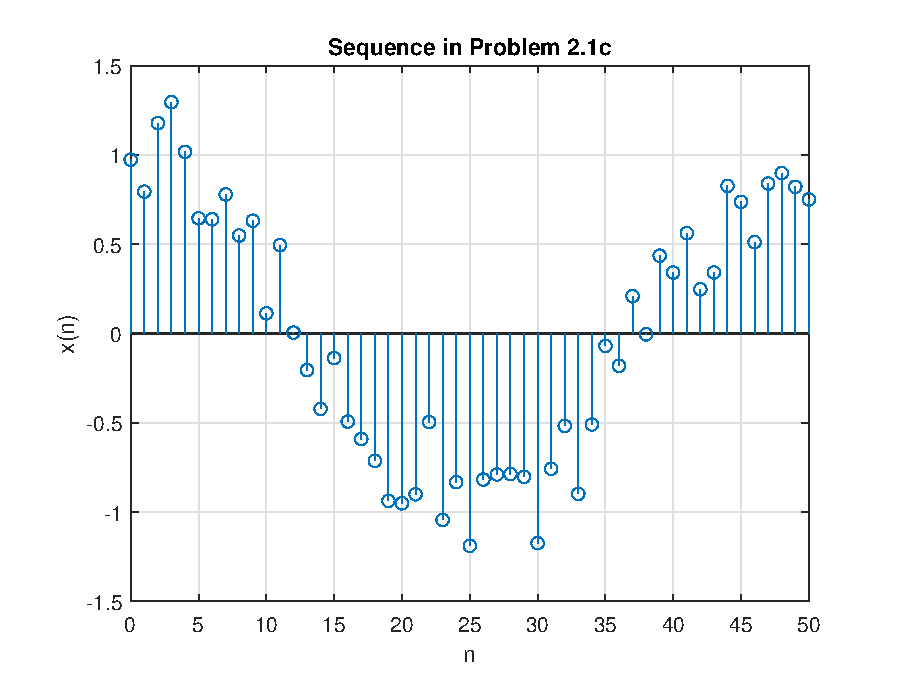
\includegraphics[width=\maxwidth{56.196688409433015em}]{figure_5.eps}
	\end{center}
	
	\begin{par}
		\begin{flushleft}
			\textbf{2) Let x(n) = \{1, 2, 3, 4, 5, 6, 7, 6, 5, 4, 3, 2, 1\}. Determine and plot the following sequence}
		\end{flushleft}
	\end{par}
	
	\begin{par}
		\begin{flushleft}
			%   a) x1(n) = 2x(n − 5) − 3x(n + 4)
		\end{flushleft}
	\end{par}
	
	\begin{matlabcode}
		n = -2:10 
	\end{matlabcode}
	\begin{matlaboutput}
		n = 1x13    
		-2    -1     0     1     2     3     4     5     6     7     8     9    10
		
	\end{matlaboutput}
	\begin{matlabcode}
		xn = [1:7,6:-1:1]
	\end{matlabcode}
	\begin{matlaboutput}
		xn = 1x13    
		1     2     3     4     5     6     7     6     5     4     3     2     1
		
	\end{matlaboutput}
	\begin{matlabcode}
		figure
		subplot(311)
		stem(xn,'linewidth',2); grid
		xlabel('n'); 
		ylabel(['x(n)']);
		
		[x11,n11] = sigshift(xn,n,5);
		[x12,n12] = sigshift(xn,n,-4);
		[x1,n1] = sigadd(2*x11,n11,-3*x12,n12);
		subplot(312)
		stem(n1,x1,'linewidth',2); grid
		title('Sequence in Example 2.a')
		xlabel('n'); 
		ylabel('x1(n)');
		
		[x21,n21] = sigfold(xn,n); 
		[x21,n21] = sigshift(x21,n21,3);
		[x22,n22] = sigshift(xn,n,2); 
		[x22,n22] = sigmult(xn,n,x22,n22);
		[x2,n2] = sigadd(x21,n21,x22,n22);
		subplot(313)
		stem(n2,x2,'linewidth',2); grid
		title(['Sequence in Example 2.b'])
		xlabel('n'); 
		ylabel('x2(n)');
	\end{matlabcode}
	\begin{center}
		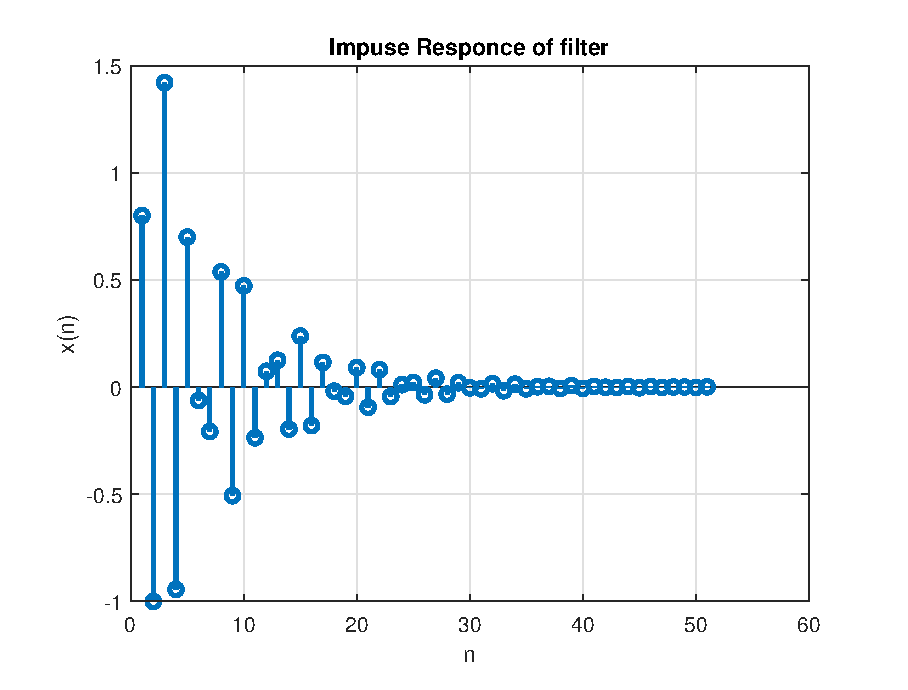
\includegraphics[width=\maxwidth{56.196688409433015em}]{figure_6.eps}
	\end{center}
	
	\begin{par}
		\begin{flushleft}
			\textbf{3) For given matrices A and B, perform matrix multiplication and scalar multiplication}
		\end{flushleft}
	\end{par}
	
	\begin{matlabcode}
		A=input('Enter the Elements of First Matrix = ');
		B=input('Enter the Elements of Second Matrix = ');
		
		[r1 c1] = size(A);
		[r2 c2] = size(B);
		if c1 ~= r2
		disp ('* not able to multiply matrices *');
		end
		
		for i = 1 : r1;
		for j = 1 : c2;
		s = 0;
		for k = 1 : c1
		A(i,k);
		B(k,j);
		s = s + A(i,k) * B(k,j);
		end
		C(i,j) = s;
		end
		end
		display(C, 'Output Matrix')
	\end{matlabcode}
	\begin{matlaboutput}
		111   126   141
		174   198   222
		237   270   303
	\end{matlaboutput}
	\begin{matlabcode}
		
		% Compare our result with a multiplication by Matlab
		display(A*B, 'Using Direct Method')
	\end{matlabcode}
	\begin{matlaboutput}
		111   126   141
		174   198   222
		237   270   303
	\end{matlaboutput}
	
	\begin{par}
		\begin{flushleft}
			\textbf{4) Generate the complex-valued signal $ \mathbf{x(n) = e^{(-0.1+j0.3)n}, -10\leq n \leq 10, }$ and plot its magnitude, phase, the real part, and the imaginary part in four separate subplots.}
		\end{flushleft}
	\end{par}
	

	
	\begin{matlabcode}
		n=-10:10
	\end{matlabcode}
	\begin{matlaboutput}
		n = 1x21    
		-10    -9    -8    -7    -6    -5    -4    -3    -2    -1     0     1     2     3     4     5     6     7     8     9    10
		
	\end{matlaboutput}
	\begin{matlabcode}
		x_n=exp((-0.1+0.3i)*n)
	\end{matlabcode}
	\begin{matlaboutput}
		x_n = 1x21 complex    
		-2.6911 - 0.3836i  -2.2237 - 1.0512i  -1.6411 - 1.5033i  -1.0166 - 1.7383i  -0.4140 - 1.7745i   0.1166 - 1.6446i   0.5406 - 1.3904i   0.8391 - 1.0574i   1.0081 - 0.6897i   1.0558 - 0.3266i   1.0000 + 0.0000i   0.8644 + 0.2674i   0.6757 + 0.4623i   0.4605 + 0.5803i   0.2429 + 0.6248i   0.0429 + 0.6050i  -0.1247 + 0.5345i  -0.2507 + 0.4287i  -0.3313 + 0.3035i  -0.3676 + 0.1738i  -0.3642 + 0.0519i
		
	\end{matlaboutput}
	\begin{matlabcode}
		figure
		subplot(221)
		stem(abs(x_n)); grid
		title('Magnitude Plot')
		xlabel('n'); 
		ylabel('|x(n)|');
		subplot(222)
		stem(angle(x_n)); grid
		title('Phase Plot')
		xlabel('n'); 
		ylabel('phase[x(n)]');
		subplot(223)
		stem(real(x_n)); grid
		title('Real Value Plot')
		xlabel('n'); 
		ylabel('Real[x(n)]');
		subplot(224)
		stem(imag(x_n)); grid
		xlabel('n'); 
		ylabel('Image[x(n)]');
		title('Imagenary Value Plot')
	\end{matlabcode}
	\begin{center}
		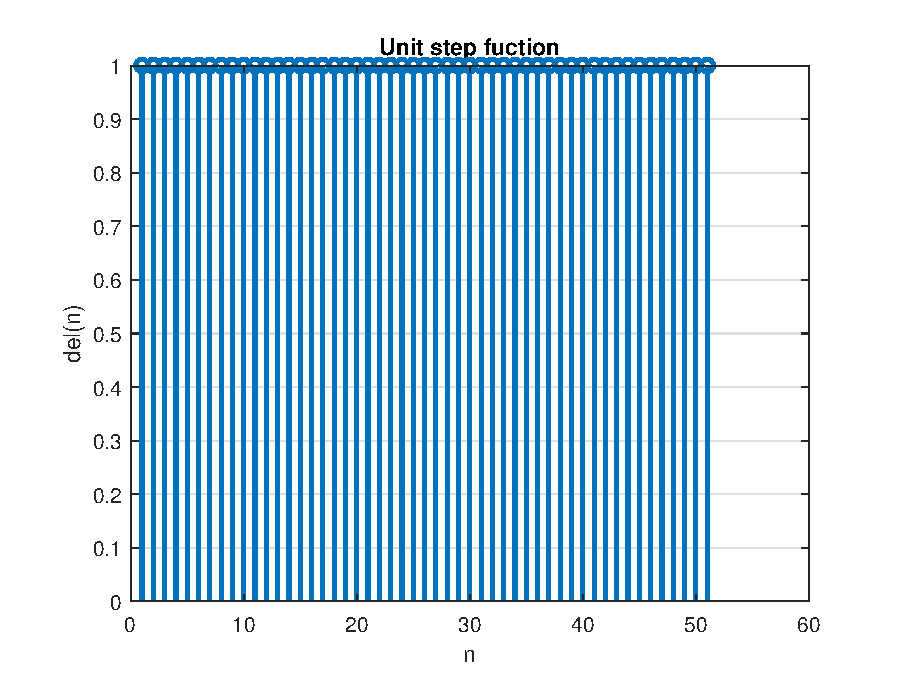
\includegraphics[width=\maxwidth{56.196688409433015em}]{figure_7.eps}
	\end{center}
	
	\begin{par}
		\begin{flushleft}
			\textbf{5) Given the following two sequences $\mathbf{x(n) = \{3, 11, 7, 0, -1, 4, 2\} , -3 \leq n \leq3; h(n) = \{2, 3, 0, -5, 2, 1\} , -1 \leq n \leq 4,}$ determine the convolution $\mathbf{y(n) = x(n)*h(n)}$ in MATLAB.}
		\end{flushleft}
	\end{par}
	
	\begin{matlabcode}
		xn=input('Enter the sequence x(n)= ');
		hn=input('Enter the sequence h(n)= ');
		m=length(xn);
		n=length(hn);
		X=[xn,zeros(1,n)];
		H=[hn,zeros(1,m)]; 
		for i=1:n+m-1
		yn(i)=0;
		for j=1:m;
		if(i-j+1>0)
		yn(i)=yn(i)+X(j)*H(i-j+1);
		else
		end
		end
		end
		display(yn, 'Output of Convolution');
	\end{matlabcode}
	\begin{matlaboutput}
		4    13    28    27    18
	\end{matlaboutput}
	\begin{matlabcode}
		yn1=conv(xn,hn);
		display(yn1, 'Output of Convolution using conv function');
	\end{matlabcode}
	\begin{matlaboutput}
		4    13    28    27    18
	\end{matlaboutput}
	\begin{matlabcode}
		
		figure
		subplot(411)
		stem(xn); grid
		title('Input sequence x(n)')
		xlabel('n')
		ylabel('x(n)')
		
		subplot(412)
		stem(hn); grid
		title('Impulse Responce h(n)')
		xlabel('n')
		ylabel('h(n)')
		
		subplot(413)
		stem(yn); grid
		title('Output of Convolution using Manual Method')
		xlabel('n')
		ylabel('y(n)')
		
		subplot(414)
		stem(yn1); grid
		title('Output of Convolution using conv function');
		xlabel('n')
		ylabel("y'(n)")
	\end{matlabcode}
	\begin{center}
		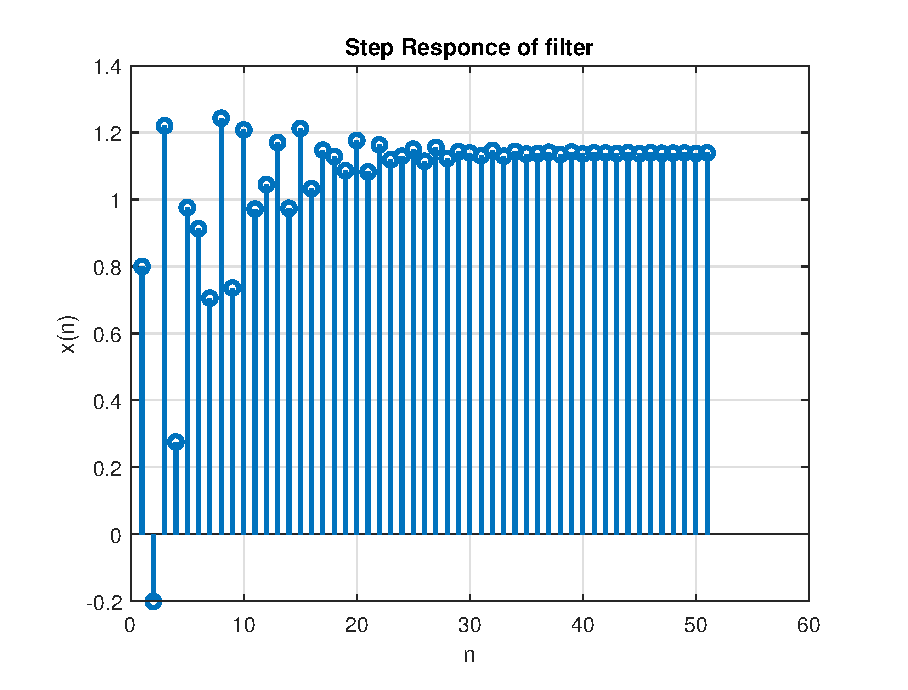
\includegraphics[width=\maxwidth{56.196688409433015em}]{figure_8.eps}
	\end{center}
	
	\begin{par}
		\begin{flushleft}
			\textbf{6) Determine the discrete-time Fourier transform of the following finite-duration sequence at 501 equispaced frequencies between $[0,\pi]: $}
		\end{flushleft}
	\end{par}
	
	\begin{par}
		\begin{flushleft}
			\textbf{a) x1(n) = \{1, 1, 1\}} 
		\end{flushleft}
	\end{par}
	
	\begin{matlabcode}
		n = 0:2; 
		x = [1 1 1];
		figure; stem(n,x); grid
		xlabel('n'); ylabel('x(n)');
		axis([-1 3 -1 2]); title('Input Sequence');
	\end{matlabcode}
	\begin{center}
		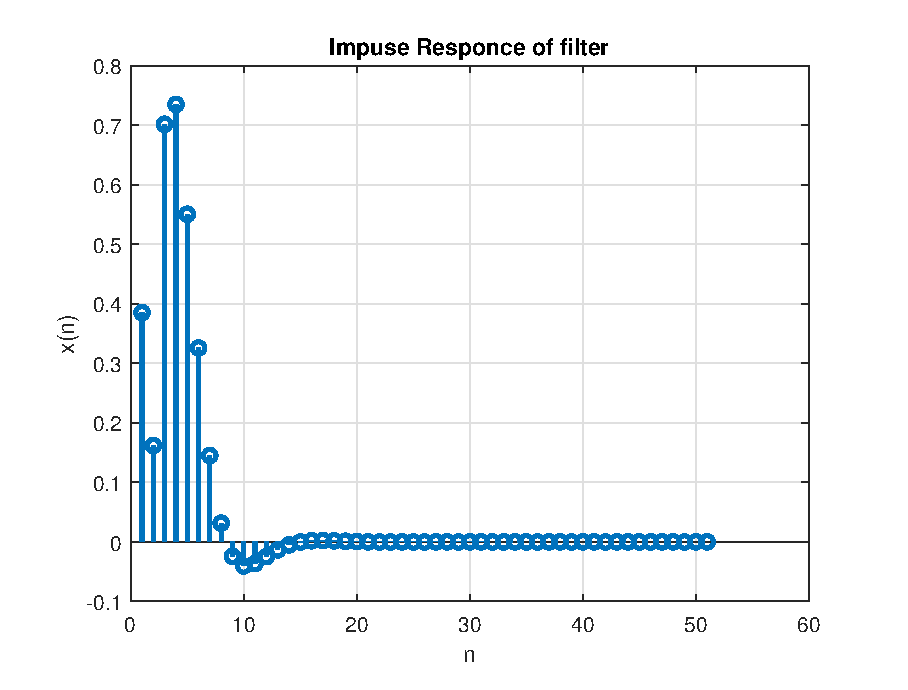
\includegraphics[width=\maxwidth{56.196688409433015em}]{figure_9.eps}
	\end{center}
	\begin{matlabcode}
		
		k = 0:500; 
		w = (pi/500)*k;  
		
		% DTFT
		X = x * (exp(-j*pi/500)) .^ (n'*k); % DTFT Calculation
		magX = abs(X); angX = angle(X);
		realX = real(X); imagX = imag(X);
		
		figure; subplot(2,2,1); plot(w/pi,magX); grid
		xlabel('frequency in pi units'); ylabel('Magnitude');
		title('Magnitude Part'); 
		
		subplot(2,2,2); plot(w/pi,angX); grid
		xlabel('frequency in pi units'); subplot(2,2,2); 
		title('Angle Part'); ylabel('Radians')
		
		subplot(2,2,3); plot(w/pi,realX); grid
		xlabel('frequency in pi units');  ylabel('Real');
		title('Real Part');
		
		subplot(2,2,4); plot(w/pi,imagX); grid
		xlabel('frequency in pi units'); ylabel('Imaginary');
		title('Imaginary Part'); 
	\end{matlabcode}
	\begin{center}
		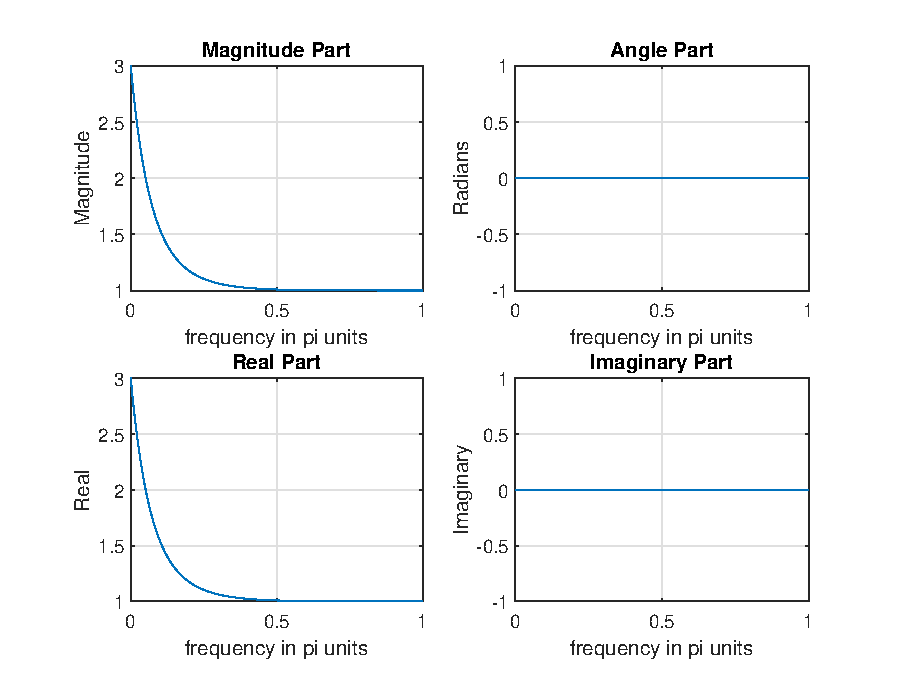
\includegraphics[width=\maxwidth{56.196688409433015em}]{figure_10.eps}
	\end{center}
	
	\begin{par}
		\begin{flushleft}
			\textbf {b) x(n) = \{1, 1, 1, 1, 0, 0, 0, 0, 1, 1, 1, 1\}} 
		\end{flushleft}
	\end{par}
	
	\begin{matlabcode}
		n = 0:11; 
		x = [1, 1, 1, 1, 0, 0, 0, 0, 1, 1, 1, 1];
		
		figure; stem(n,x); grid
		xlabel('n'); ylabel('x(n)');
		axis([-1 12 -1 2]); title('Input Sequence');
	\end{matlabcode}
	\begin{center}
		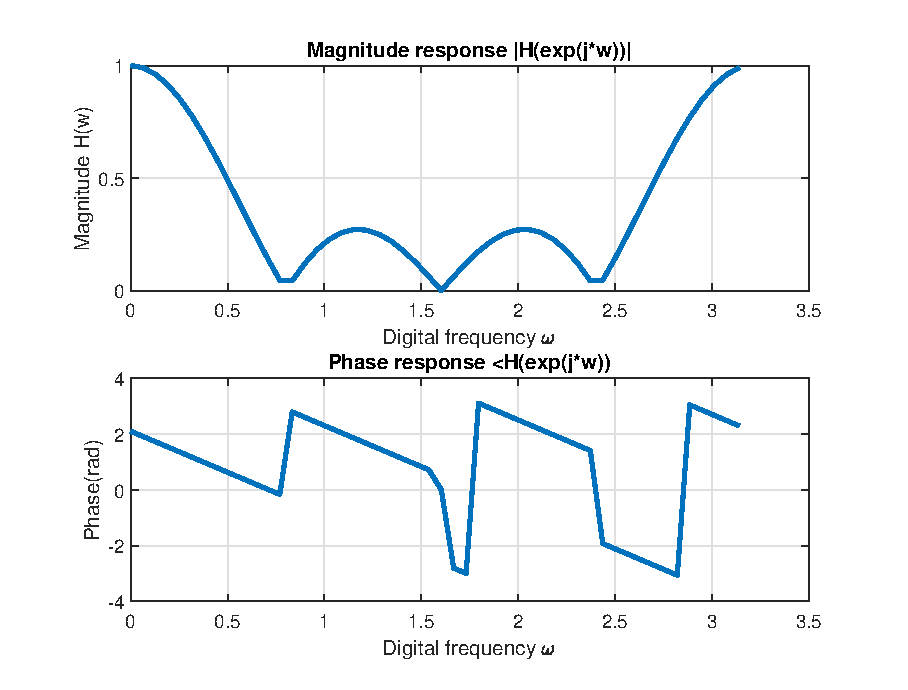
\includegraphics[width=\maxwidth{56.196688409433015em}]{figure_11.eps}
	\end{center}
	\begin{matlabcode}
		
		k = 0:500; 
		w = (pi/500)*k;  
		
		% DTFT
		X = x * (exp(-j*pi/500)) .^ (n'*k); % DTFT Calculation
		magX = abs(X); angX = angle(X);
		realX = real(X); imagX = imag(X);
		
		figure; subplot(2,2,1); plot(w/pi,magX); grid
		xlabel('frequency in pi units'); ylabel('Magnitude');
		title('Magnitude Part'); 
		
		subplot(2,2,2); plot(w/pi,angX); grid
		xlabel('frequency in pi units'); subplot(2,2,2); 
		title('Angle Part'); ylabel('Radians')
		
		subplot(2,2,3); plot(w/pi,realX); grid
		xlabel('frequency in pi units');  ylabel('Real');
		title('Real Part');
		
		subplot(2,2,4); plot(w/pi,imagX); grid
		xlabel('frequency in pi units'); ylabel('Imaginary');
		title('Imaginary Part'); 
	\end{matlabcode}
	\begin{center}
		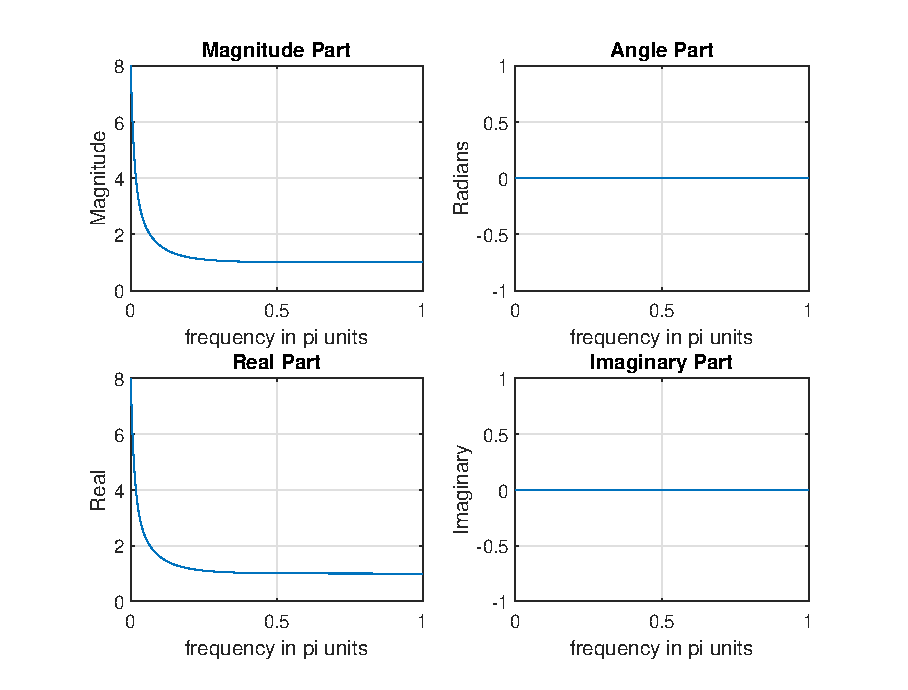
\includegraphics[width=\maxwidth{56.196688409433015em}]{figure_12.eps}
	\end{center}
	
	\begin{par}
		\begin{flushleft}
			c) x2(n) = \{1, 2, 3, 4, 5\} 
		\end{flushleft}
	\end{par}
	
	\begin{matlabcode}
		n = 0:4; 
		x = [1:5];
		
		figure; stem(n,x); grid
		xlabel('n'); ylabel('x(n)');
		axis([-1 5 -1 6]); title('Input Sequence');
	\end{matlabcode}
	\begin{center}
		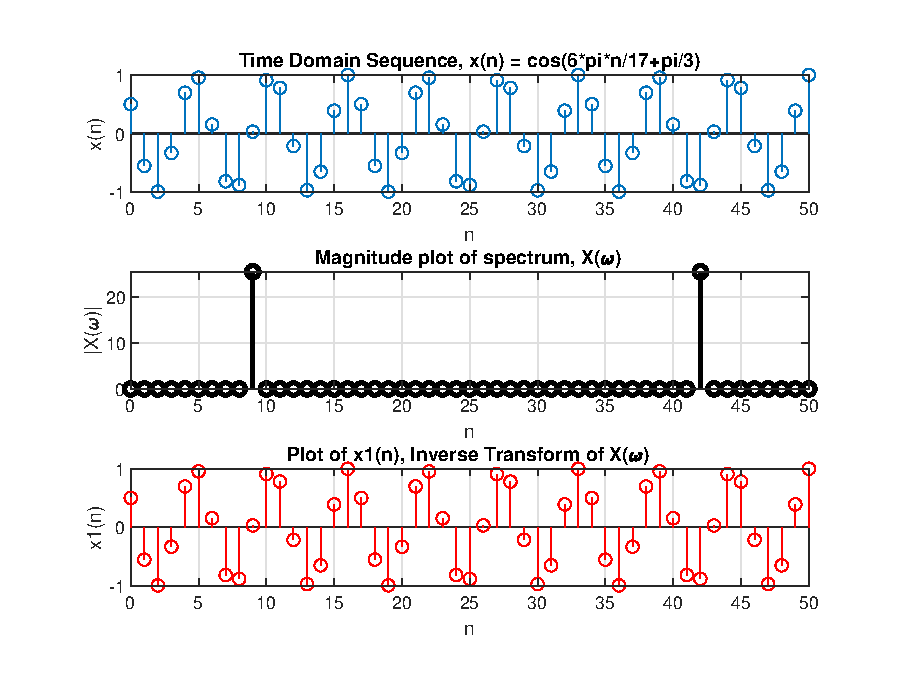
\includegraphics[width=\maxwidth{56.196688409433015em}]{figure_13.eps}
	\end{center}
	\begin{matlabcode}
		
		k = 0:500; % DTFT Points
		w = (pi/500)*k;  
		
		% DTFT
		X = x * (exp(-j*pi/500)) .^ (n'*k); % DTFT Calculation
		magX = abs(X); angX = angle(X);
		realX = real(X); imagX = imag(X);
		
		figure; subplot(2,2,1); plot(w/pi,magX); grid
		xlabel('frequency in pi units'); ylabel('Magnitude');
		title('Magnitude Part'); 
		
		subplot(2,2,2); plot(w/pi,angX); grid
		xlabel('frequency in pi units'); subplot(2,2,2); 
		title('Angle Part'); ylabel('Radians')
		
		subplot(2,2,3); plot(w/pi,realX); grid
		xlabel('frequency in pi units');  ylabel('Real');
		title('Real Part');
		
		subplot(2,2,4); plot(w/pi,imagX); grid
		xlabel('frequency in pi units'); ylabel('Imaginary');
		title('Imaginary Part'); 
	\end{matlabcode}
	\begin{center}
		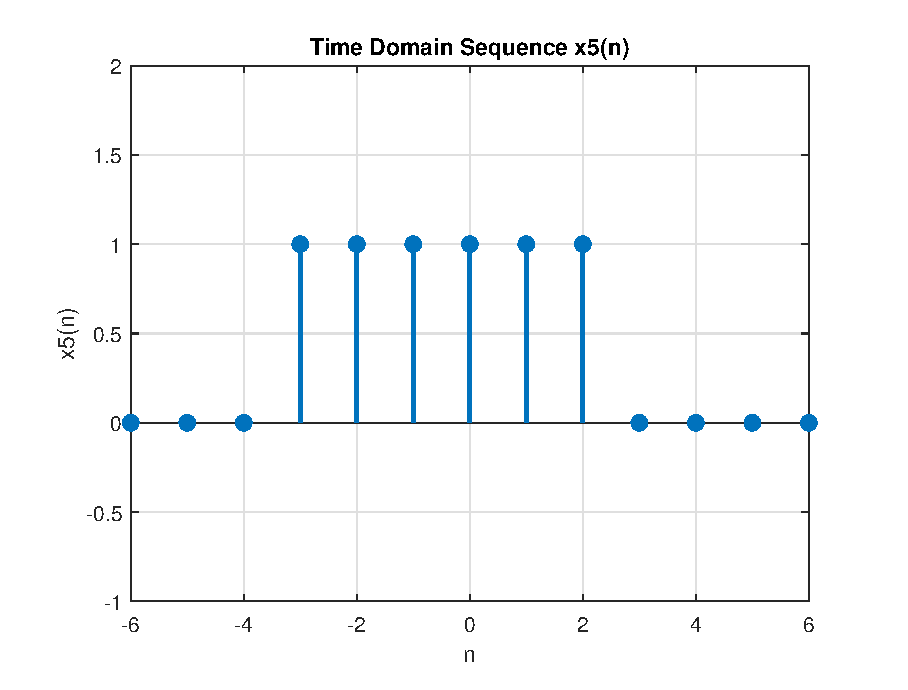
\includegraphics[width=\maxwidth{56.196688409433015em}]{figure_14.eps}
	\end{center}
	
	\begin{par}
		\begin{flushleft}
			%d) x3(n) = \{sin(πn/5)\} , n = \{1, 2, ....10\}
		\end{flushleft}
	\end{par}
	
	\begin{matlabcode}
		n = 1:10; 
		x = sin(pi*n/5);
		
		figure; stem(n,x); grid
		xlabel('n'); ylabel('x(n)');
		axis([0 11 -2 2]); title('Input Sequence');
	\end{matlabcode}
	\begin{center}
		\includegraphics[width=\maxwidth{56.196688409433015em}]{figure_15.eps}
	\end{center}
	\begin{matlabcode}
		
		k = 0:500; % DTFT Points
		w = (pi/500)*k;  
		
		% DTFT
		X = x * (exp(-j*pi/500)) .^ (n'*k); % DTFT Calculation
		magX = abs(X); angX = angle(X);
		realX = real(X); imagX = imag(X);
		
		figure; subplot(2,2,1); plot(w/pi,magX); grid
		xlabel('frequency in pi units'); ylabel('Magnitude');
		title('Magnitude Part'); 
		
		subplot(2,2,2); plot(w/pi,angX); grid
		xlabel('frequency in pi units'); subplot(2,2,2); 
		title('Angle Part'); ylabel('Radians')
		
		subplot(2,2,3); plot(w/pi,realX); grid
		xlabel('frequency in pi units');  ylabel('Real');
		title('Real Part');
		
		subplot(2,2,4); plot(w/pi,imagX); grid
		xlabel('frequency in pi units'); ylabel('Imaginary');
		title('Imaginary Part'); 
	\end{matlabcode}
	\begin{center}
		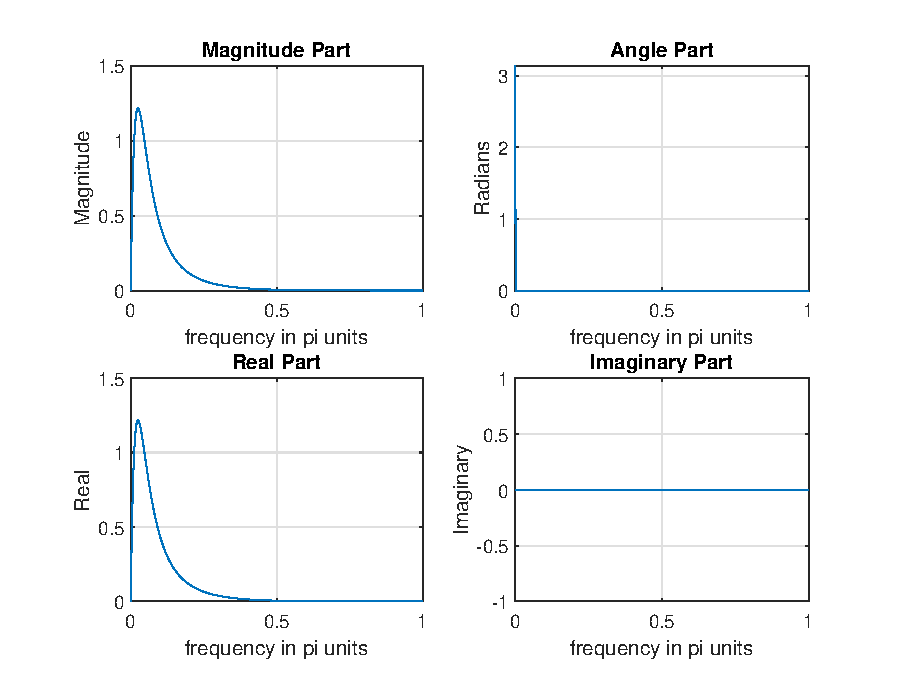
\includegraphics[width=\maxwidth{56.196688409433015em}]{figure_16.eps}
	\end{center}
	
\end{document}